% --
% machine learning

\section{Neural Networks for KWS}
\sectionheader{Neural Networks for KWS}

\begin{frame}
  \frametitle{Neural Network approaches}
  \begin{itemize}
    \item Convolutional Neural Networks (CNNs)
    \begin{itemize}
      \item MFCCs as input features
      \item simple network architecutures with different striding properties adapted from \cite{Sainath2015}
    \end{itemize}
    \item Generative Adversarial Neural Networks (GANs) \cite{Goodfellow2014}
    \begin{itemize}
      \item used to improve the classification performance of equivalent CNN models
    \end{itemize}
    \item Wavenets \cite{Oord2016}
    \begin{itemize}
      \item raw audio data as input features
      \item no feature extraction
    \end{itemize}
  \end{itemize}
\end{frame}

\begin{frame}
  \frametitle{Fully Connected Layer}
  \begin{columns}
    \begin{column}{0.45\textwidth}
      \begin{itemize}
        \item Output with activation $h$:
        \begin{equation*}
          \footnotesize
          \begin{aligned}
            \bm{z} = h(W \bm{x} + \bm{b})
          \end{aligned}
        \end{equation*}
        {\scriptsize with $\bm{x} \in \R^n$, $\bm{z} \in \R^m$, $\bm{b} \in \R^m$.}
        \vspace{0.2cm}
        \item Amount of Params:
        \begin{equation*}
          \footnotesize
          \begin{aligned}
            m \cdot n + m
          \end{aligned}
        \end{equation*}
        \item Amount of Operations:
        \begin{equation*}
          \footnotesize
          \begin{aligned}
            \mathcal{T}(W \bm{x} + \bm{b}) \approx 2 (m \cdot n) + m
          \end{aligned}
        \end{equation*}     
      \end{itemize}
    \end{column}
    \begin{column}{0.55\textwidth}
      \vspace{0.75cm}
      \centering
      \begin{figure} 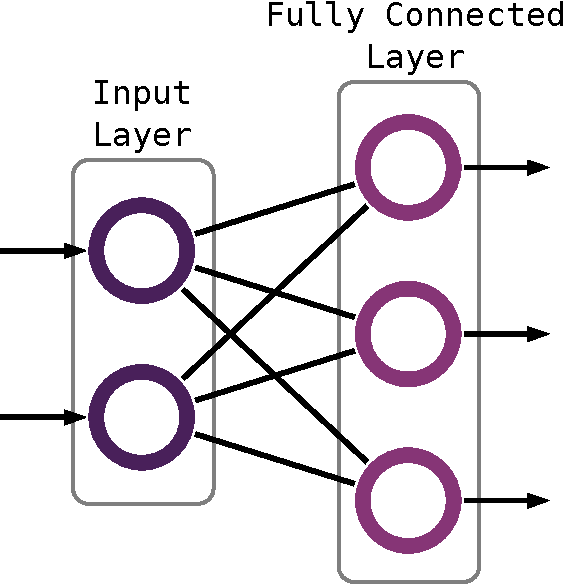
\includegraphics[width=0.55\textwidth]{../4_nn/figs/nn_theory_fc.pdf} \end{figure}
      \vfill
    \end{column}
  \end{columns}
\end{frame}

\begin{frame}
  \frametitle{Convolutional Layer}
  \begin{columns}
    \begin{column}{0.5\textwidth}
      \begin{itemize}
        \item j-th output channel $o_j$:
        \begin{equation*}
          \footnotesize
          o_j = \sum_{i} k_{i, j} \ast x_i,
        \end{equation*}
        \footnotesize
        with $x_i$ as i-th input channel and $k_{i, j}$ as kernel.   
      \end{itemize}
    \end{column}
    \begin{column}{0.5\textwidth}
      \centering
      \begin{figure} 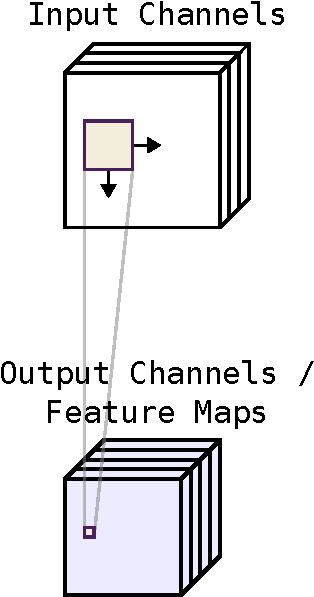
\includegraphics[width=0.45\textwidth]{./figs/nn_theory_cnn_scheme.pdf} \end{figure}
      \vfill
    \end{column}
  \end{columns}
\end{frame}

\begin{frame}
  \frametitle{Convolutional Layer Example}
  \vspace{0.2cm}
  \begin{figure} 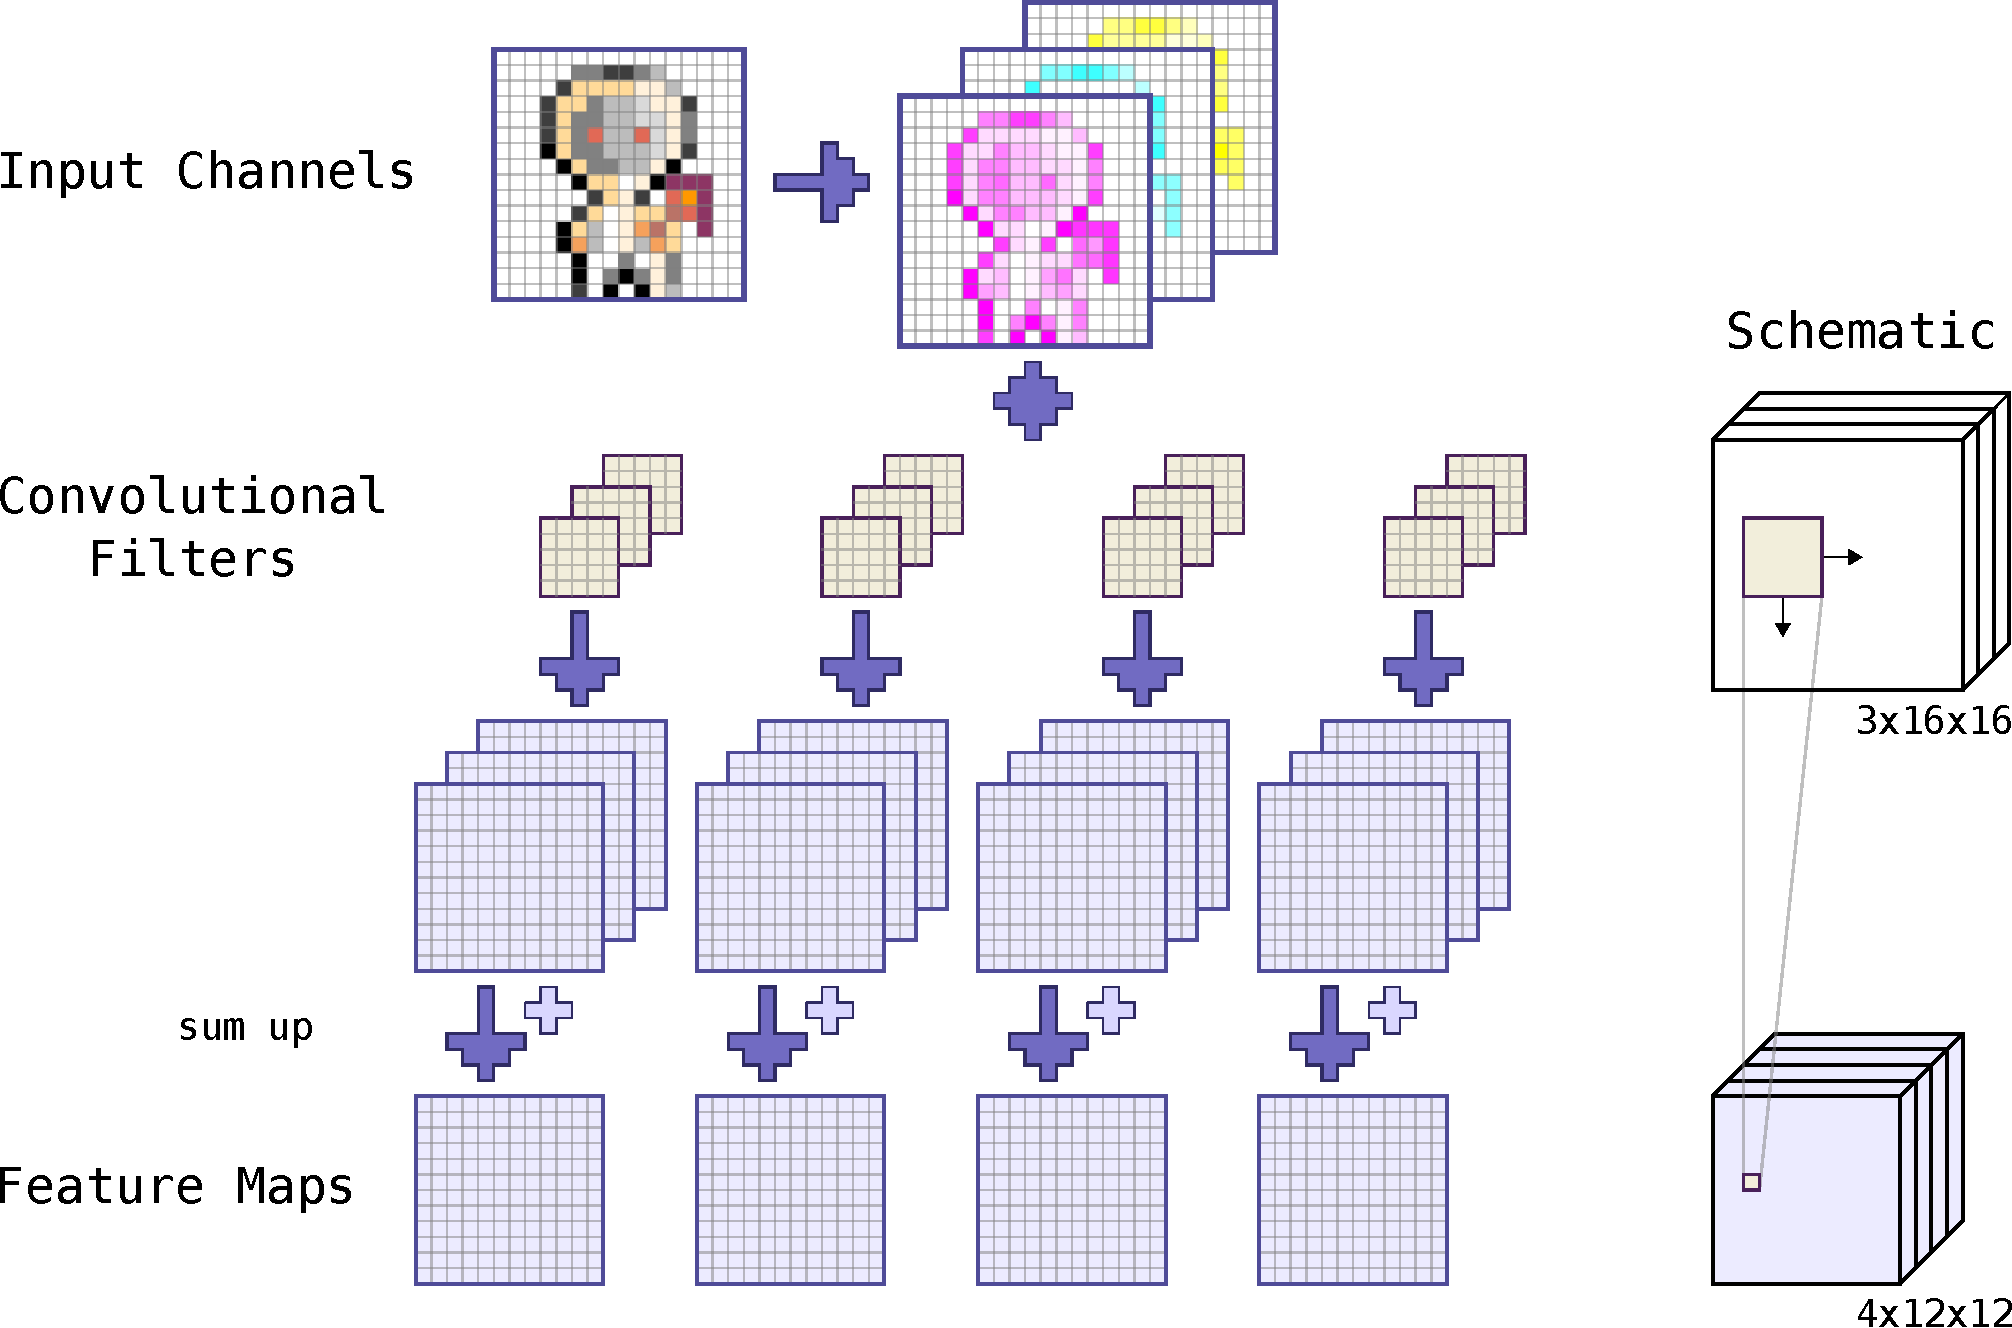
\includegraphics[width=0.8\textwidth]{../4_nn/figs/nn_theory_cnn_basics.pdf} \end{figure}
\end{frame}

\begin{frame}
  \frametitle{Striding properties of CNNs}
  \begin{itemize}
    \item striding of the conv. filters (kernels) from the first conv. layers of all three CNN models:
  \end{itemize}
  \hspace{1cm}
  \scalebox{0.75}
  {
    \begin{tikzpicture}
      \node at (0, 0) (ktrad) [inner sep=0] {
\includegraphics[width=0.5\textwidth]{./figs/real_right_sample.png}};
      \node [below=of ktrad, inner sep=0] (kfstride) {
\includegraphics[width=0.5\textwidth]{./figs/real_right_sample.png}};
      \node [below=of kfstride, inner sep=0] (kjim) {
\includegraphics[width=0.5\textwidth]{./figs/real_right_sample.png}};

      % fstride
      \draw [color=neonlightblue, line width=1.5pt] (ktrad.north west) rectangle ++(62pt, -0.45cm);
      \draw [->, line width=1.0pt, color=neonlightblue] ($(ktrad.west) + (65pt, 13pt)$) -- ++(8pt, 0);
      \draw [->, line width=1.0pt, color=neonlightblue] ($(ktrad.south) + (-48pt, 0.8cm)$) -- ++(0, -8pt);

      % fstride
      \draw [color=neonlightblue, line width=1.5pt] (kfstride.north west) rectangle ($(kfstride.north east) + (0, -0.9cm)$);
      \draw [->, line width=1.0pt, color=neonlightblue] ($(kfstride.south) + (0, 0.35cm)$) -- ++(0, -8pt);

      % fstride
      \draw [color=neonlightblue, line width=1.5pt] (kjim.north west) rectangle ($(kjim.south west) + (62pt, 0)$);
      \draw [->, line width=1.0pt, color=neonlightblue] ($(kjim.west) + (65pt, 0)$) -- ++(8pt, 0);

      % text
      \node at (ktrad.west) [xshift=-2pt, anchor=east] {conv-trad};
      \node at (kfstride.west) [xshift=-2pt, anchor=east] {conv-fstride};
      \node at (kjim.west) [xshift=-2pt, anchor=east] {conv-jim};
    \end{tikzpicture}
  }
\end{frame}

\begin{frame}
  \frametitle{Traditional Network (conv-trad)}
  \begin{itemize}
    \item Layer Structure: Conv.: 2 + 1 max. pool, FC: 3 
    \item Num. Params: \textbf{\num{68396}}
    \item Num. Operations: \textbf{\SI{3770.98}{\kilo\ops}}
  \end{itemize}
  \begin{figure} 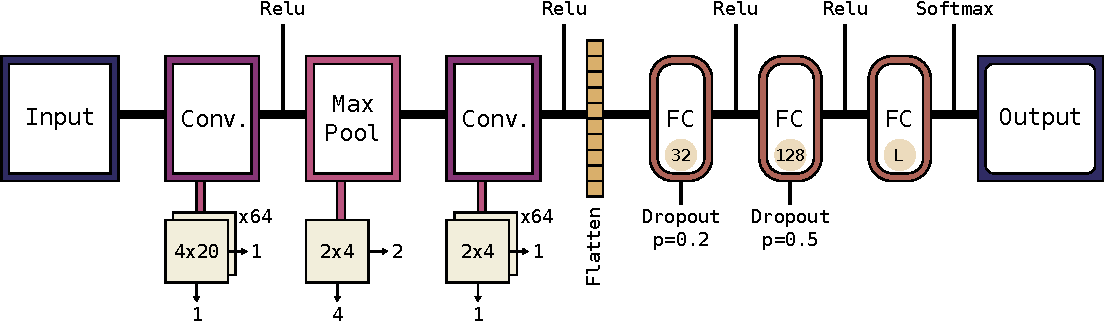
\includegraphics[height=0.35\textheight]{../4_nn/figs/nn_arch_cnn_trad.pdf} \end{figure}
\end{frame}

\begin{frame}
  \frametitle{Frequency Striding Network (conv-fstride)}
  \begin{itemize}
    \item Layer Structure: Conv.: 1, FC: 4
    \item Num. Params: \textbf{\num{47426}} 
    \item Num. Operations: \textbf{\SI{137.75}{\kilo\ops}}
  \end{itemize}
  \begin{figure} 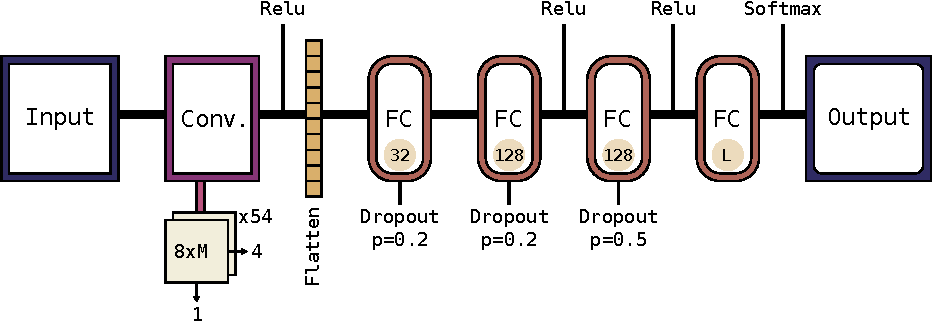
\includegraphics[height=0.35\textheight]{../4_nn/figs/nn_arch_cnn_fstride.pdf} \end{figure}
\end{frame}

\begin{frame}
  \frametitle{Time Striding Network(conv-jim)}
  \begin{itemize}
    \item Layer Structure: Conv.: 2, FC: 3
    \item Num. Params: \textbf{\num{29804}}
    \item Num. Operations: \textbf{\SI{862.40}{\kilo\ops}}
  \end{itemize}
  \begin{figure} 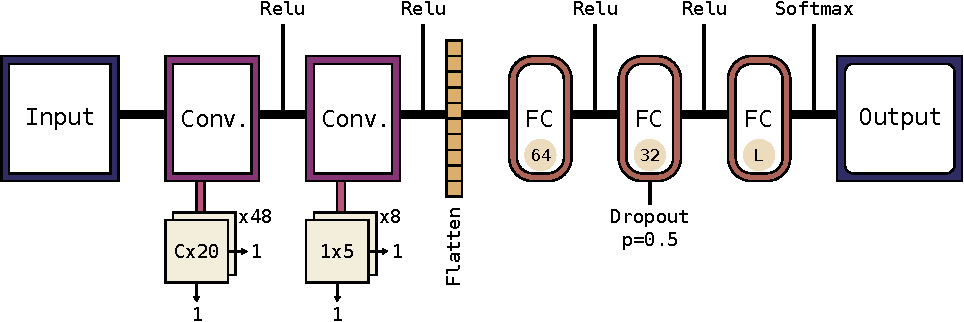
\includegraphics[height=0.35\textheight]{../4_nn/figs/nn_arch_cnn_jim.pdf} \end{figure}
\end{frame}


\begin{frame}
  \frametitle{GANs}
  \begin{itemize}
    \item consist of two adversarial networks:
    \begin{itemize}
      \footnotesize
      \item Discriminator (D): classify images to fake or real  $D: \mathcal{X} \mapsto [0, 1]$ .
      \item Generator (G): produce new data examples $G: \mathcal{Z} \mapsto \mathcal{X}$.
    \end{itemize}
    \begin{tikzpicture} 
      \node at (0, 0) (g) {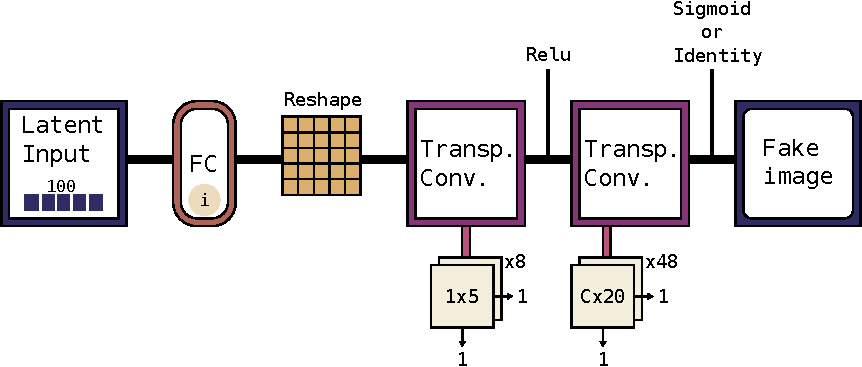
\includegraphics[width=0.4\textwidth]{../4_nn/figs/nn_arch_adv_g_jim.pdf}};
      \node at (g.east)[yshift=0.1cm] (vs) [anchor=west, font=\bf] {vs.};
      \node at (vs.east)[yshift=-0.2cm] (d) [anchor=west] {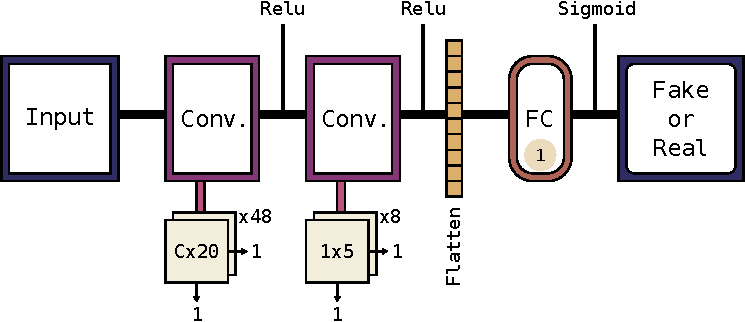
\includegraphics[width=0.35\textwidth]{../4_nn/figs/nn_arch_adv_d_jim.pdf}};
      \node at (vs.south)[yshift=-0.3cm] (sample) [anchor=north, rectangle, draw=blue!25!black, inner sep=2pt, line width=1pt] {
\includegraphics[width=0.10\textwidth]{./figs/nn_adv_generated_sample.png}};
      % lines
      \draw [<-] [color=blue!25!black, line width=0.5pt] (sample.west) -- ++(-0.20cm, 0cm) -- ++(0, 0.4cm);
      \draw [->] [color=blue!25!black, line width=0.5pt] (sample.east) -- ++(0.20cm, 0cm) -- ++(0, 0.4cm);
      % text above
      \node at (g.north west) [xshift=0.6cm, yshift=-0.1cm, anchor=north east] {\scriptsize G};
      \node at (d.north west) [xshift=0.6cm, yshift=0.1cm, anchor=north east] {\scriptsize D};
    \end{tikzpicture}
    \vspace{0.2cm}
    \item Min-Max Solution for the Game between G and D:
  \end{itemize}
  \begin{equation*}
    \footnotesize
    \begin{aligned}
      \underset{G}{\min} \, \underset{D}{\max} \, V(D, G) = \quad & \E_{\bm{x} \sim p_{data}(\bm{x})}\left[ \log D(\bm{x}) \right] + \\
      & \E_{\bm{z} \sim p_{\bm{z}}(\bm{z})}\left[ \log (1 - D(G(\bm{z}))) \right],
    \end{aligned}
  \end{equation*}
\end{frame}

\begin{frame}
  \frametitle{GAN training losses}
  \begin{itemize}
    \item binary cross entropy loss $l$:
    \begin{equation*}
      \footnotesize
      \begin{aligned}
        l(x_i, y_i) = y_i \cdot \log x_i + (1 - y_i) \cdot \log (1 - x_i)
      \end{aligned}
    \end{equation*}
    \item loss of D ($y_r$: real-, $y_f$: fake-label):
    \begin{equation*}
      \footnotesize
      \begin{aligned}
        l_D(x_i, z_i, G) = l(D(x_i), y_r) + l(D(G(z_i)), y_f)
      \end{aligned}
    \end{equation*}
    \item loss of G:
    \begin{equation*}
      \footnotesize
      \begin{aligned}
        l_G(z_i, D) =  l(D(G(z_i)), y_r)
      \end{aligned}
    \end{equation*}
    \item loss of G with similarity term ($s$ is cosine similarity):
    \begin{equation*}
      \footnotesize
      \begin{aligned}
        l_G(x_i, z_i, D) =  l(D(G(z_i)), y_r) + \lambda \left(1 - \frac{1}{C} \sum_{c=0}^{C} s(\hat{\bm{e}}_c^T x_i , \hat{\bm{e}}_c^T G(z_i)) \right),
      \end{aligned}
    \end{equation*}
  \end{itemize}
\end{frame}


\begin{frame}
  \frametitle{Adversarial Label Training}
  \begin{itemize}
    \item individual training instances on label subsets:
  \end{itemize}
  \begin{figure} 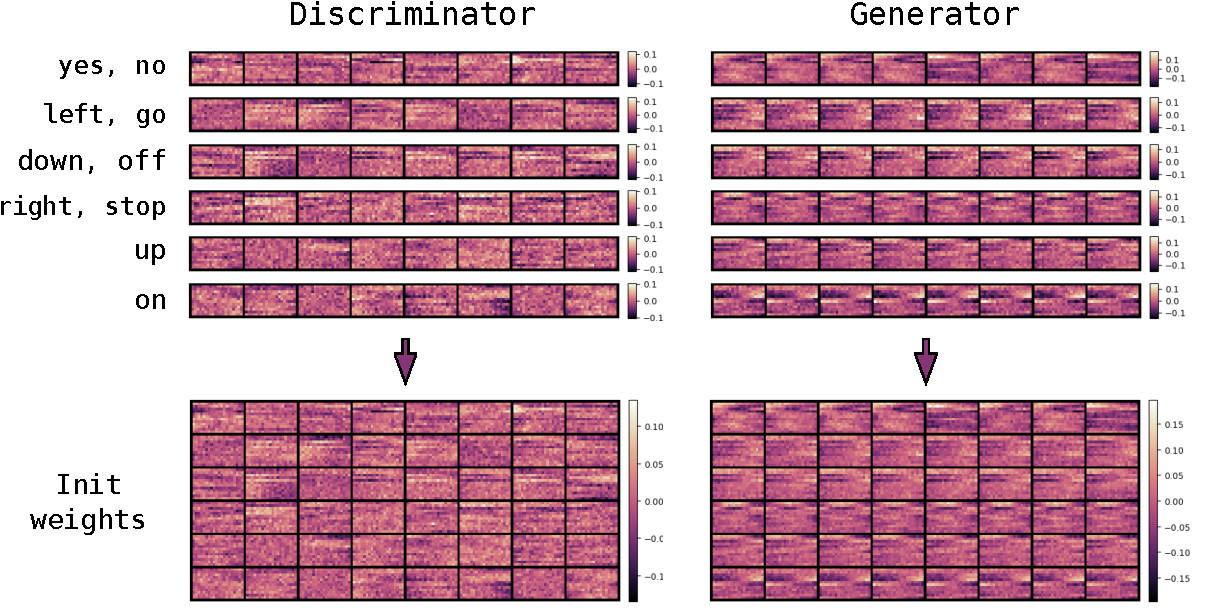
\includegraphics[height=0.7\textheight]{../4_nn/figs/nn_adv_label_scheme.pdf} \end{figure}
\end{frame}


\begin{frame}
  \frametitle{Adversarial Label Training}
  \begin{itemize}
    \item training on label \enquote{right} without similarity term:
  \end{itemize}
    \begin{tikzpicture} 
      \node at (0, 0) (a) {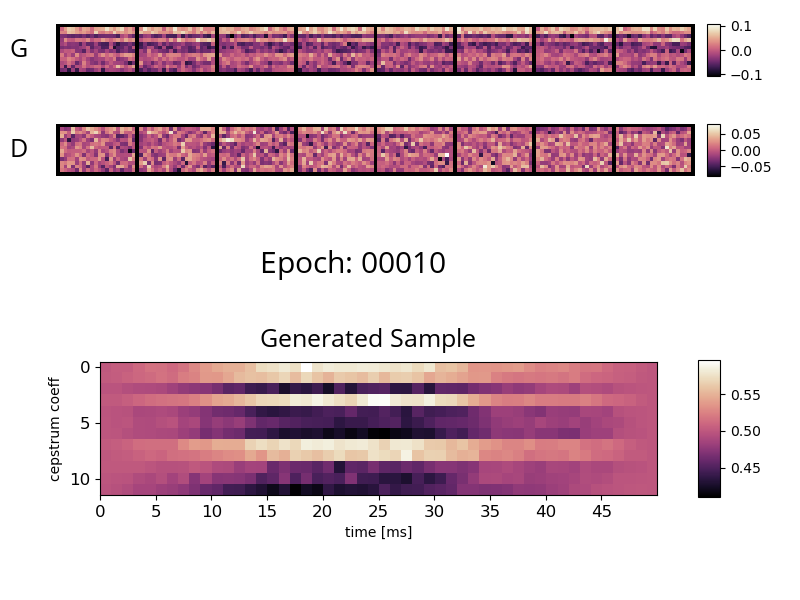
\includegraphics[width=0.4\textwidth]{./figs/adv_experimental_ep-10}};
      \node at (a.east)[xshift=0.2cm] (b) [anchor=west] {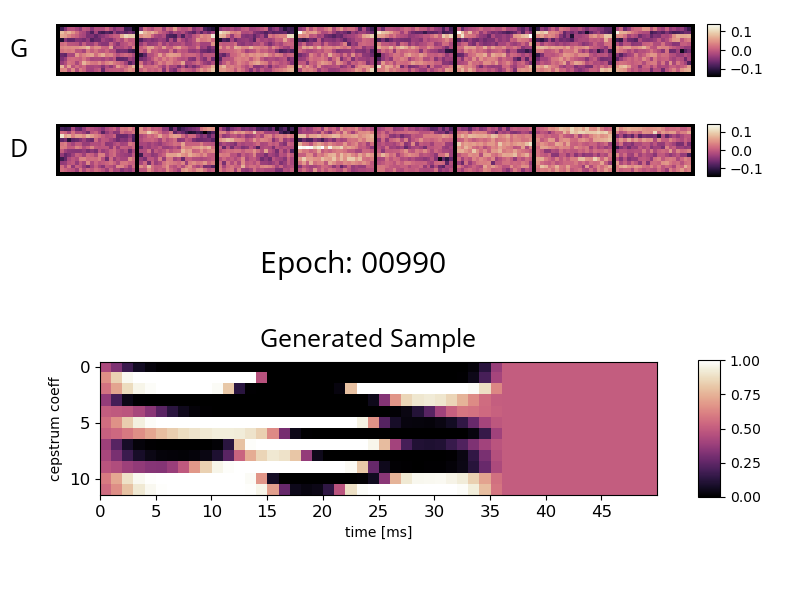
\includegraphics[width=0.4\textwidth]{./figs/adv_experimental_ep-990}};
      \node at (a.south) (c) [anchor=north] {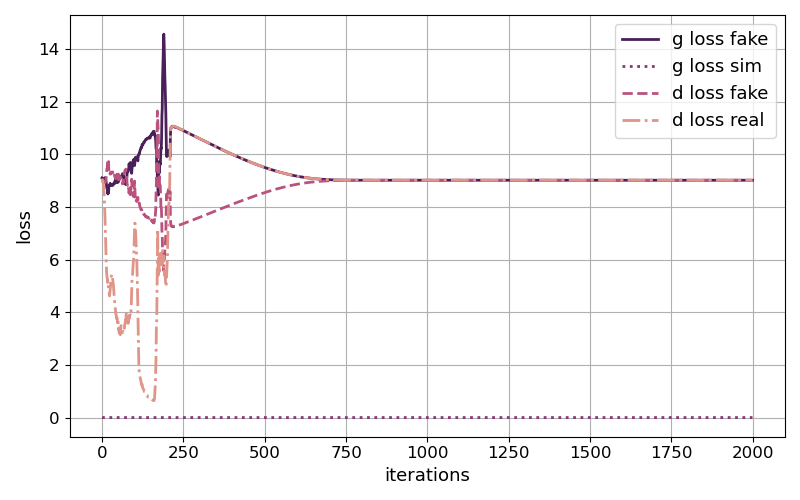
\includegraphics[width=0.4\textwidth]{./figs/adv_experimental_loss}};
      % lines
      \draw [->] [color=blue!25!black, line width=1.5pt] (a.east) -- ++(6pt, 0cm);
    \end{tikzpicture}
\end{frame}

\begin{frame}
  \frametitle{Adversarial Label Training}
  \begin{itemize}
    \item training on label \enquote{right} with similarity term:
  \end{itemize}
    \begin{tikzpicture} 
      \node at (0, 0) (a) {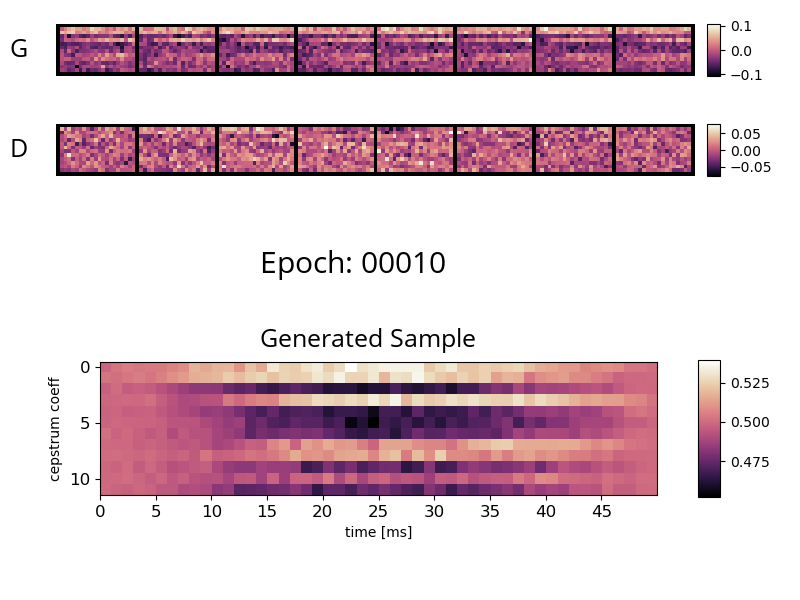
\includegraphics[width=0.4\textwidth]{./figs/adv_conv-jim_ep-10}};
      \node at (a.east)[xshift=0.2cm] (b) [anchor=west] {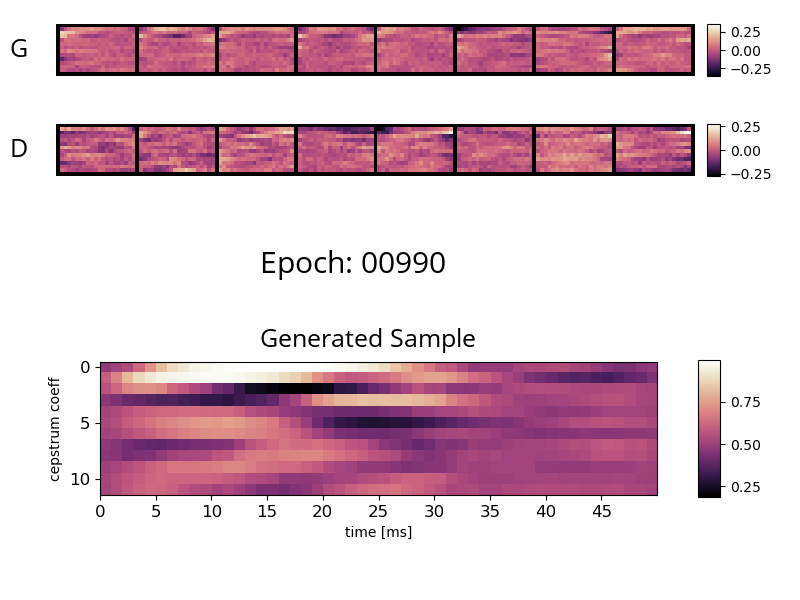
\includegraphics[width=0.4\textwidth]{./figs/adv_conv-jim_ep-990}};
      \node at (a.south) (c) [anchor=north] {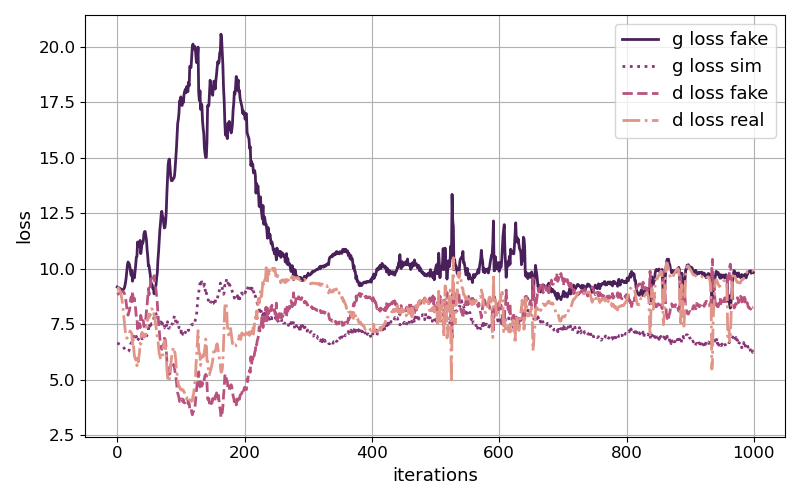
\includegraphics[width=0.4\textwidth]{./figs/adv_conv-jim_loss}};
      % lines
      \draw [->] [color=blue!25!black, line width=1.5pt] (a.east) -- ++(6pt, 0cm);
    \end{tikzpicture}
\end{frame}





\begin{frame}
  \frametitle{Wavenets}
  \begin{itemize}
    \item Perform  on raw audio data ($\SI{1}{\second}$ = 16000 features)
    \item Key Techniques: 
    \begin{itemize}
      \item dilated convolutions
      \item quantization
    \end{itemize}
    \item Residual block schematic:
  \end{itemize}
  \vspace{-0.2cm}
  \begin{figure} 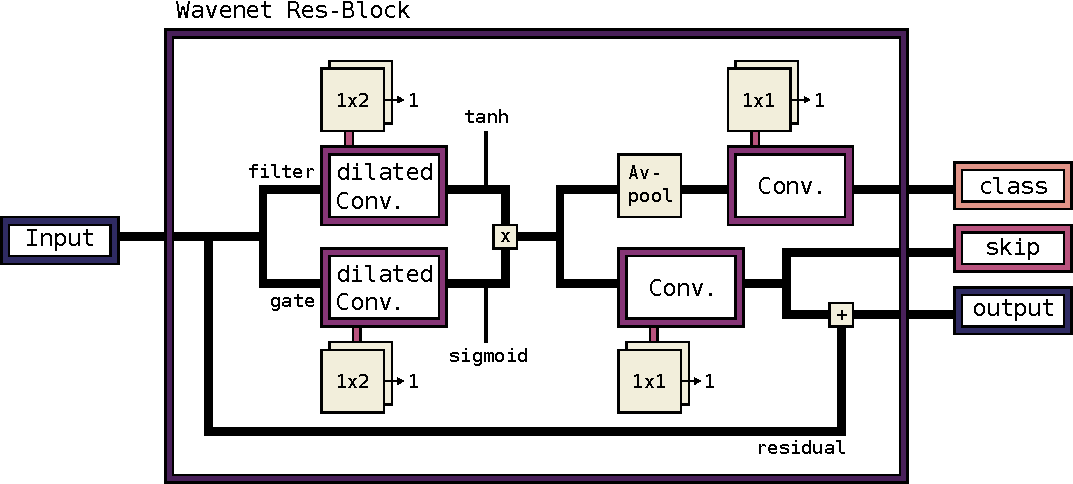
\includegraphics[height=0.35\textheight]{../4_nn/figs/nn_arch_wavenet_block.pdf} \end{figure}
\end{frame}

\begin{frame}
  \frametitle{Wavenet Architecture}
  \begin{itemize}
    \item Num. Params: \textbf{\num{33509}}
    \item Num. Operations: \textbf{\SI{36695.02}{\kilo\ops}}
  \end{itemize}
  \vspace{-0.2cm}
  \begin{figure} 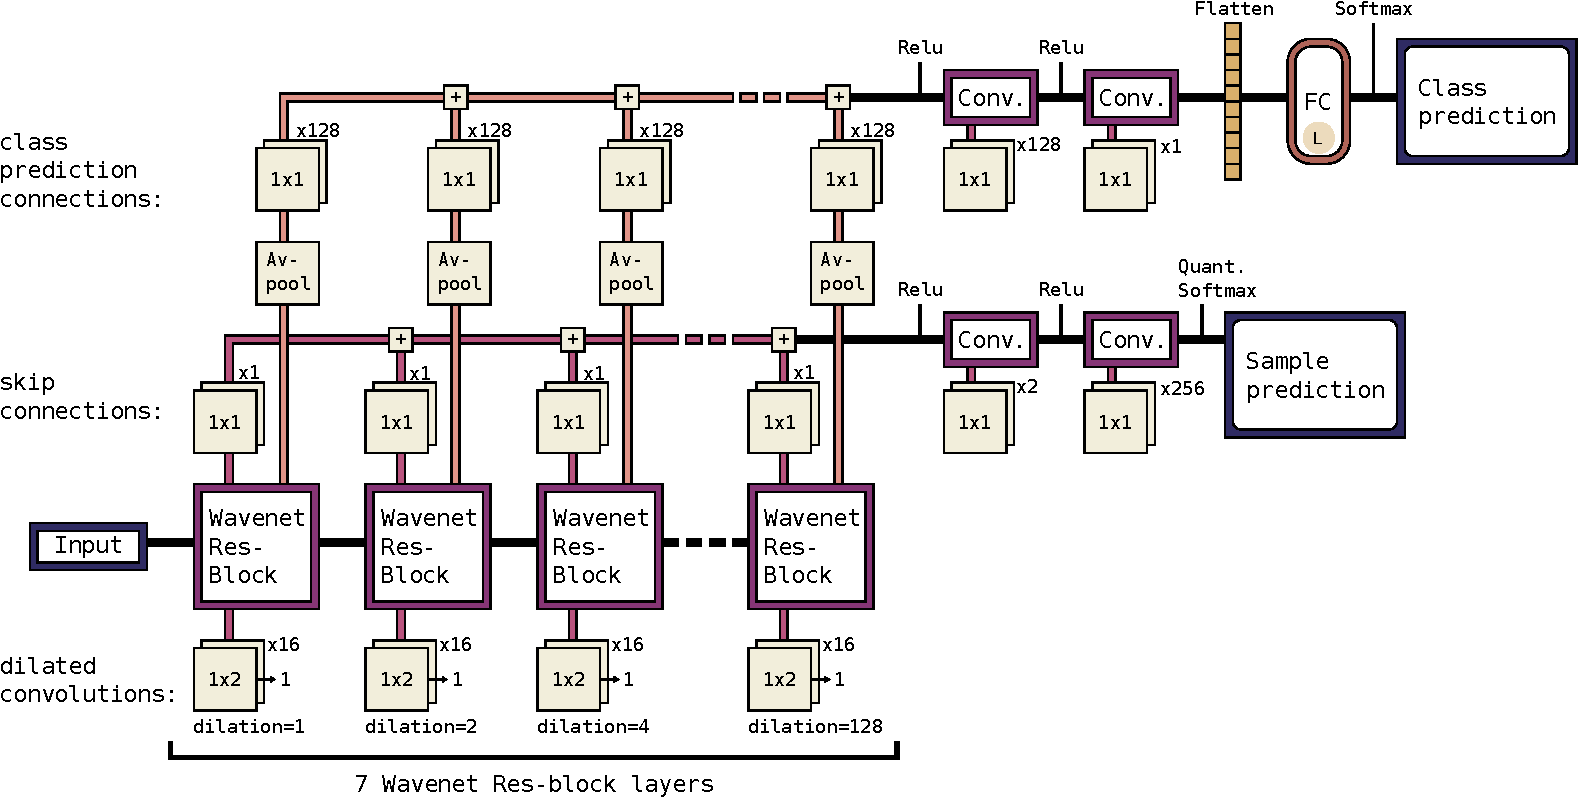
\includegraphics[height=0.6\textheight]{../4_nn/figs/nn_arch_wavenet_all.pdf} \end{figure}
\end{frame}